\documentclass[11pt]{article}

\usepackage[margin=1in]{geometry}
\usepackage{amsmath,amssymb,amsthm}
\usepackage{graphicx}
\usepackage[hidelinks]{hyperref}

\newtheorem{theorem}{Theorem}

\newcommand{\SEP}{\mathrm{SEP}}
\newcommand{\ellp}{\ell_p}
\newcommand{\Lp}{L_p}

\begin{document}

\begin{center}
{\Large Literature status: separation growth of \(\ell_p\), \(p>2\)}

\medskip
{\small Run \texttt{fa\_banach\_001}; source arXiv:2112.11523}
\end{center}

\section*{Source question}

Naor's \emph{Extension, separation and isomorphic reverse isoperimetry}
defines \(\SEP^n(M)\) to be the supremum of the separation moduli of subsets
of a metric space \(M\) with cardinality at most \(n\).  In Section 1.7.6,
after discussing dimension reduction, it asks the following question for
\(\ell_p\), \(p>2\).

\begin{figure}[h]
\centering

\includegraphics[width=\textwidth]{figures/open_question_crop.png}
\caption{arXiv:2112.11523, page 44: Question 83 on separation growth of
\(\ell_p\), \(p>2\).}
\end{figure}

The ambitious part of the question asks whether, for every fixed
\(p\in(2,\infty)\),
\[
  \SEP^n(\ell_p)\lesssim_p \sqrt{\log n}.
\]
This would imply the preceding nontrivial-growth question
\(\SEP^n(\ell_p)/\log n\to 0\).

\section*{Supporting literature status}

Naor and Ren's later paper \emph{Euclidean embedding, randomized clustering,
and Lipschitz extension for finite and doubling subsets of \(L_p\) when
\(p>2\)} explicitly cites this question as \cite[Question 83]{Naor2024} and
proves the sharp fixed-\(p\) answer for \(L_p\).

\begin{figure}[h]
\centering

\includegraphics[width=\textwidth]{figures/supporting_answer_crop.png}
\caption{arXiv:2502.10543, page 11: explicit reference to
\cite[Question 83]{Naor2024} and Theorem 1.10.}
\end{figure}

\begin{figure}[h]
\centering
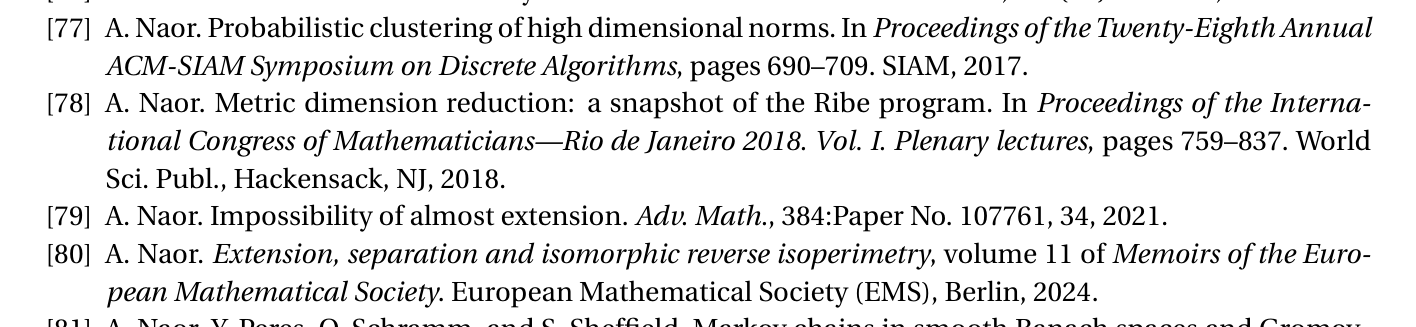
\includegraphics[width=\textwidth]{figures/supporting_references_crop.png}
\caption{arXiv:2502.10543, page 59: bibliography entries [77] and [80],
identifying the 2017 SODA question and Naor's 2024 monograph.}
\end{figure}

\section*{Proof intuition}

Question 83 was difficult because for \(p\neq 2\) one cannot simply reduce a
finite subset of \(\ell_p\) to logarithmic dimension by a Hilbert-style
dimension-reduction lemma.  Naor--Ren instead prove a direct partition theorem
for finite subsets of the ambient \(L_p\) space.  Since \(\ell_p\) is an
isometric subspace of \(L_p\), any finite subset of \(\ell_p\) inherits the
same randomized partition bound from the larger space.

\section*{The literature answer}

\begin{theorem}
For every fixed \(p\in(2,\infty)\),
\[
  \SEP^n(\ell_p)\lesssim_p \sqrt{\log n}.
\]
Consequently,
\[
  \lim_{n\to\infty}\frac{\SEP^n(\ell_p)}{\log n}=0.
\]
Thus Question 83 of \cite{Naor2024} has an affirmative answer for each fixed
\(p>2\).
\end{theorem}

\begin{proof}
Naor--Ren's Theorem 1.10 \cite{NaorRen} states that, for every
\((p,n)\in(2,\infty)\times\mathbb{N}\),
\[
  \sqrt{\log n}\lesssim \SEP^n(L_p)\lesssim p^2\sqrt{\log n}.
\]
The upper bound is the needed part.

Embed \(\ell_p\) isometrically into an \(L_p\) space, for example by
representing a sequence as a step function on pairwise disjoint measurable
sets with the usual normalization.  If \(S\subset \ell_p\) and \(|S|\le n\),
then \(S\) is also an \(n\)-point subset of \(L_p\), and therefore
\[
  \SEP(S)\le \SEP^n(L_p)\lesssim p^2\sqrt{\log n}.
\]
Taking the supremum over all such \(S\subset \ell_p\) gives
\[
  \SEP^n(\ell_p)\le \SEP^n(L_p)\lesssim p^2\sqrt{\log n}.
\]
For fixed \(p\), the right hand side is \(o(\log n)\), which also answers the
nontrivial-growth part of Question 83.
\end{proof}

\section*{Verification notes and limitations}

This packet is a literature-status identification, not a new proof from the
run.  The supporting paper explicitly says that the sharp
\(\sqrt{\log n}\) question was asked in \cite{Naor2017} and
\cite{Naor2024}, and more specifically identifies the latter as
\cite[Question 83]{Naor2024}.  Its bibliography identifies
\cite{Naor2024} as \emph{Extension, separation and isomorphic reverse
isoperimetry}.

The answer is for fixed \(p>2\).  Naor--Ren note that, when \(p\) is allowed
to vary with \(n\), the range
\(\sqrt[4]{\log n}\lesssim p=o(\log n)\) remains open.  This packet also does
not address the other reverse-isoperimetry, shape-optimization, or
Schatten-class conjectures in \cite{Naor2024}.

Before promotion, the run lightweight indexes were searched for arXiv:2112.11523,
the title phrase, ``separation growth'', ``SEP\^{}n'', and related terms.  No
existing exact packet or attempt was found.  The only nearby registry hit was
the distinct arXiv:1506.04398 / arXiv:2502.10543 packet on Lipschitz extension
upper bounds.

\section*{Human review recommendation}

Treat arXiv:2112.11523 Question 83 as already answered affirmatively, in its
fixed-\(p>2\) and \(\sqrt{\log n}\) form, by arXiv:2502.10543.  Keep the other
questions in the source paper separate.

\begin{thebibliography}{9}

\bibitem{Naor2017}
A. Naor,
\emph{Probabilistic clustering of high dimensional norms},
Proceedings of the Twenty-Eighth Annual ACM-SIAM Symposium on Discrete
Algorithms, 690--709, SIAM, 2017.

\bibitem{Naor2024}
A. Naor,
\emph{Extension, separation and isomorphic reverse isoperimetry},
Memoirs of the European Mathematical Society, vol. 11,
European Mathematical Society, Berlin, 2024; arXiv:2112.11523.

\bibitem{NaorRen}
A. Naor and K. Ren,
\emph{Euclidean embedding, randomized clustering, and Lipschitz extension for
finite and doubling subsets of \(L_p\) when \(p>2\)},
arXiv:2502.10543.

\end{thebibliography}

\end{document}
